%% Methods + Results + floats for the PGG-punishment paper (\input by main.tex).

\section{Methods}

\subsection{The public-goods game with punishment}
We replicate the public-goods game with costly peer punishment of \textcite{herrmann2008antisocial}. Four players are matched as partners for the whole game and play ten periods. Each period every player receives a fresh endowment of 20 tokens and contributes an integer amount between 0 and 20 to a group project with a marginal per-capita return of 0.4, so that each contributed token returns 0.4 tokens to all four members. In treatment~N players only contribute. In treatment~P the contribution stage is followed by a costly punishment stage in which each player may assign 0--10 deduction points to each other member; every point costs the punisher one token and removes three tokens from the target, the canonical 1:3 cost ratio. To block cross-period identity tracking, the other members are re-labelled every period. There is no communication, and we run ten independent groups per cell. Following \textcite{herrmann2008antisocial}, we classify punishment by the contribution deviation between target and punisher: punishment of a target who contributed equal to or more than the punisher (deviation $\geq 0$) is \emph{antisocial}, whereas punishment of a lower contributor (deviation $<0$) is punishment of free-riding.

\subsection{Agents, models and protocol}
Each agent is an instruction-tuned LLM that receives a single natural-language prompt comprising a brief of the game rules, the history of play so far, and a disposition or society block, after which it reasons briefly and emits a parseable decision line---\texttt{CONTRIBUTION = X} in the contribution stage and \texttt{DEDUCT: A=a B=b C=c} in the punishment stage. Within each stage, all four agents' decisions are collected in a single lockstep batch so that play is genuinely simultaneous. The protocol is built on the FAIRGAME multi-agent framework \parencite{fairgame2025}. We serve three open-weight instruction-tuned models, Qwen2.5-7B-Instruct \parencite{qwen2025}, Gemma-2-9B-it \parencite{gemma2024} and Llama-3.1-8B-Instruct \parencite{llama2024}, via vLLM at temperature 0.8 with a fixed seed to make runs reproducible; all simulations were executed offline on a single RTX PRO 6000. Exact model identifiers, decoding settings and per-condition game counts are listed in the electronic supplementary material. Each game is crossed with five languages (English, French, Arabic, Chinese, Vietnamese) and four dispositional prompts (neutral, cooperative, selfish, vengeful); we additionally cross sixteen society personas drawn from the participant cities of \textcite{herrmann2008antisocial} (Boston, Copenhagen, Zurich, St.\,Gallen, Nottingham, Bonn, Seoul, Melbourne, Chengdu, Minsk, Samara, Dnipropetrovsk, Muscat, Istanbul, Riyadh and Athens), each rendered as a neutral ``You are a participant from <City>, <Country>.'' persona that carries no behavioural stereotype.

\subsection{Measures and analysis}
For each game we record the mean per-period contribution (of 20 tokens) and, in treatment~P, the punishment assigned by each member. The antisocial share is the antisocial deduction points divided by all deduction points, and we additionally bin punishment expenditure by the contribution deviation between target and punisher. The punishment-institution effect is summarised as the contribution difference P$-$N and tested with the Mann--Whitney $U$ test on the ten per-group means. All human benchmark values are the published summary statistics of \textcite{herrmann2008antisocial} (per-pool mean contributions over the sixteen participant pools; grand means 8.6 and 12.9 tokens in the N and P treatments). Because two of the central results are nulls, we quantify evidence \emph{for} them rather than relying on failure to reject: the P$-$N contrast is accompanied by a two-one-sided-tests (TOST) Welch equivalence test \parencite{lakens2018equivalence} whose smallest effect size of interest is half the human grand-mean gain ($\pm 2.14$ tokens) and by a JZS Bayes factor $\mathrm{BF}_{01}$ \parencite{rouder2009bayesian}, and each model's antisocial-punishment--cooperation coupling is tested directly against the human $\rho\approx-0.90$ with a Fieller-corrected Fisher-$z$ test. The cross-societal signature of \textcite{herrmann2008antisocial} is assessed with the Spearman rank correlation between per-society antisocial punishment and mean contribution, and the alignment of the model's geography of cooperation with the human ordering across the sixteen societies is evaluated with Spearman rank correlations and Wilcoxon signed-rank tests against the human pool means. We report bias-corrected effect sizes (Hedges $g$ and the rank-biserial correlation for the P$-$N contrast) with 95\%\ confidence intervals and Holm--Bonferroni-adjusted $p$-values; the full effect-size tables, the per-society breakdown and the dispositional analysis appear in the electronic supplementary material. Throughout, we log the \texttt{parse\_fallback} (format non-compliance) rate for every cell and report it as a joint data-quality and fairness signal.

\section{Results}

\begin{table*}[t]
\caption{Mean contribution (of 20 tokens) in the faithful baseline (English
prompt, neutral disposition) without (N) and with (P) a punishment stage, the
punishment effect $\Delta=\bar c_P-\bar c_N$, and the antisocial share of all
punishment (points aimed at members who contributed equal to or more than the
punisher). The human reference is the 16-pool grand mean of Herrmann
\textit{et al.}\ \cite{herrmann2008antisocial}, where punishment raised
cooperation ($\Delta\approx+4.3$) and antisocial punishment, though present, was
a minority of expenditure in most pools. $p$ from a two-sided Mann--Whitney $U$
test on the ten per-group means (P vs N).}
\label{tab:baseline}
\centering
\begin{tabular}{lccccc}
\toprule
Player & Contrib.\ N & Contrib.\ P & $\Delta$ (P$-$N) & $p$ & Antisocial share \\
\midrule
Human \cite{herrmann2008antisocial} & 8.6 & 12.9 & $+4.3$ & --- & minority\textsuperscript{*} \\
Qwen2.5-7B   & $14.26 \pm 0.48$ & $13.90 \pm 0.51$ & $-0.36$ & 0.71   & 59\% \\
Gemma-2-9B   & $13.41 \pm 0.37$ & $9.86  \pm 0.37$ & $-3.55$ & $<$0.001 & 55\% \\
Llama-3.1-8B & $10.67 \pm 0.45$ & $10.75 \pm 0.43$ & $+0.08$ & 0.91   & 54\% \\
\bottomrule
\end{tabular}
\\[2pt]
{\footnotesize \textsuperscript{*}In Herrmann \textit{et al.}\ the antisocial
share varied widely across societies but prosocial punishment of free-riding
dominated in most Western pools.}
\end{table*}

\begin{figure*}[t]
\centering
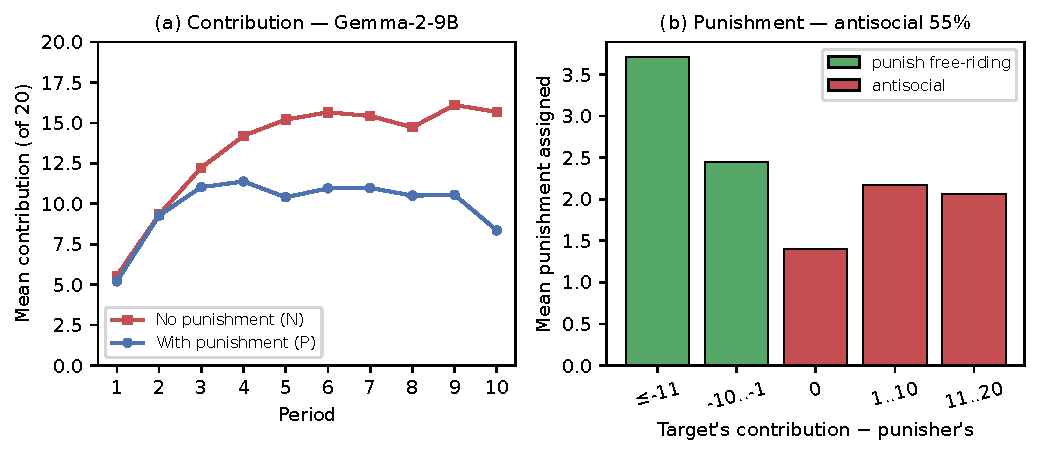
\includegraphics[width=\textwidth]{figures/fig1_punishment.pdf}
\caption{Punishment dynamics for Gemma-2-9B. (\textit{a}) Mean contribution per
period without (N) and with (P) punishment: the punishment treatment lies
\textit{below} the no-punishment baseline, the opposite of the human result that
punishment sustains cooperation. (\textit{b}) Mean punishment assigned by the
contribution deviation of the target relative to the punisher; green bars are
prosocial punishment of free-riding, red bars are antisocial punishment of equal
or higher contributors, which accounts for 55\% of all expenditure.}
\label{fig:punishment}
\end{figure*}

In the contribution-only treatment (N) all three models sustained substantial cooperation, with baseline mean contributions of $14.26\pm0.48$ (Qwen), $13.41\pm0.37$ (Gemma) and $10.67\pm0.45$ (Llama) tokens of the 20-token endowment (table~\ref{tab:baseline})---comfortably above the human grand-mean of $8.6$ tokens \cite{herrmann2008antisocial}. The diagnostic test, however, is whether adding a costly peer-punishment stage (treatment P) lifts cooperation, the central result of the punishment literature \cite{fehr2002altruistic,herrmann2008antisocial}. It does not. The within-model difference $\mathrm{P}-\mathrm{N}$ was $-0.36$ tokens for Qwen, $-3.55$ for Gemma and $+0.08$ for Llama, against a human grand-mean gain of approximately $+4.3$ tokens (from $8.6$ under N to $12.9$ under P). For two of the three models the punishment institution thus left cooperation flat or, in Gemma's case, drove it significantly \emph{down} (Mann--Whitney $p<0.001$; the per-period $\mathrm{N}>\mathrm{P}$ trajectory is shown in figure~\ref{fig:punishment}a), while for Qwen the small decline was not significant ($p=0.71$) and Llama's near-zero change likewise did not differ from chance ($p=0.91$). These two nulls are supported positively rather than by mere non-significance: TOST equivalence tests establish that the institutional effect for Qwen and Llama is reliably smaller than half the human gain (TOST $p=0.010$ and $0.002$), with JZS Bayes factors favouring no treatment difference ($\mathrm{BF}_{01}=2.3$ and $2.5$), whereas for Gemma the same analyses decisively reject both the null and equivalence in the direction of a harmful institution ($\mathrm{BF}_{01}=1.8\times10^{-4}$, overwhelming evidence for a difference; TOST $p=0.99$). The institutional responsiveness that makes punishment informative about human conditional cooperation is therefore absent.

The punishment that the models did assign, moreover, was substantially antisocial. Classifying each deduction by the contribution deviation between target and punisher, antisocial punishment---points aimed at a target who contributed equal to or more than the punisher (deviation $\geq 0$)---accounted for $59\%$, $55\%$ and $54\%$ of all points for Qwen, Gemma and Llama respectively, rivalling the most punitive human participant pools \cite{herrmann2008antisocial}. Yet the deviation-binned structure of that punishment (figure~\ref{fig:punishment}b) reveals that the models differ sharply in whether they retain the human-like logic of punishing deeper free-riding more harshly. Only Gemma reproduced the monotone gradient, escalating from $2.45$ points in the mild-free-riding bin to $3.71$ points for the most extreme free-riders (deviation $\leq -11$) while sparing equal contributors ($1.40$ points at deviation $0$). Qwen and Llama, by contrast, punished almost uniformly across deviation bins, meting out comparable deductions to free-riders and cooperators alike: Qwen ranged only from $2.15$ to $2.78$ points and Llama from $2.53$ to $2.86$ points across the full deviation spectrum, punishing equal-or-higher contributors ($2.29$ and $2.60$ points at deviation $0$) nearly as hard as the worst free-riders. The behavioural surface of punishment is present, but for two models the underlying targeting logic that distinguishes prosocial from antisocial sanctioning is not.

\begin{figure*}[t]
\centering
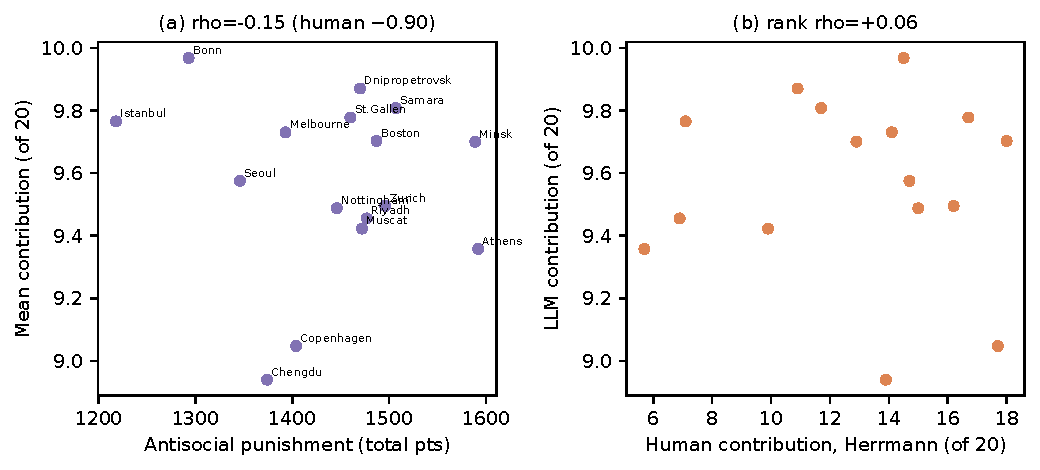
\includegraphics[width=\textwidth]{figures/fig2_cross.pdf}
\caption{The cross-societal signature is not reproduced. (\textit{a}) Per-society
antisocial punishment versus mean contribution for the 16 city personas
(Gemma-2-9B): the strong negative association seen in humans
(Spearman $\rho\approx-0.90$) is absent ($\rho=-0.15$). (\textit{b}) LLM versus
human \cite{herrmann2008antisocial} mean contribution across the same societies:
the model compresses every society into a $\sim$1-token band and does not
reproduce the human ranking (rank $\rho=+0.06$).}
\label{fig:cross}
\end{figure*}

Most consequentially, the cross-societal signature that makes Herrmann's study diagnostic of culturally heterogeneous norms fails to emerge. In the human data, pools where antisocial punishment is prevalent are those where cooperation is low, yielding a strong negative rank correlation of approximately $-0.90$ between per-society antisocial punishment and mean contribution \cite{herrmann2008antisocial}. Across our sixteen neutral city personas this relationship was effectively flat: the antisocial-versus-cooperation Spearman correlation was $-0.09$ for Qwen, $-0.15$ for Gemma and $+0.30$ for Llama (figure~\ref{fig:cross}a)---in Llama's case of the opposite sign. Each of these couplings differs significantly from the human $\rho\approx-0.90$ over the same sixteen pools (Fieller-corrected Fisher-$z$ tests; $p=0.0006$, $0.0011$ and $p<10^{-4}$, respectively). The accompanying ``geography of cooperation'' also collapsed: society personas shifted contribution by only about one token, compressing all sixteen cities into a narrow band rather than reproducing the broad human cross-cultural spread (figure~\ref{fig:cross}b). The models did not even rank the societies as humans do, with LLM-versus-human cross-societal rank correlations of just $+0.33$ (Qwen), $+0.06$ (Gemma) and $+0.17$ (Llama), and the overall level of cooperation differed from the human pools for two of the three models (Wilcoxon $p=0.005$ for Gemma and $p=0.025$ for Llama, mean LLM$-$human differences of $-3.30$ and $-2.47$ tokens; Qwen did not differ, $p=0.67$). Thus, even where the models do punish, contribute and engage in antisocial sanctioning, the culturally structured preference heterogeneity that is the scientific payload of the original experiment is missing.
